\chapter{Cycle 3: Simulation}
\graphicspath{{figures}}

% To Do:
%   - Hierarchy diagram
%   - Do more testing


\section{Brief Outline}

    This cycle will address the simulation of electrical circuits as well as how the user will interact with creation of circuits as well as information being communicated to the user.
    
    Will draw the hierarchy diagram in LaTeX at some point

    % Include hierarchy diagram here

    % Should probably draw it out and plan it on paper first

    % and have a REAL idea of what I want to complete in this cycle

    % Will have to address the circtuit simulation aspect
    % and linking all the previous cycles together and how it will all work 


    \subsection{Success Criteria}
        See \autoref{tbl:succ-crit-c3}.

\section{Design}

    \subsection{Data Structures}
        The most important data structure to be designed is that of the `circuit' itself. 
        By looking at real-life circuits and circuit diagrams, they clearly share a lot of features with a graph, and considering that current only flows in one direction, a directed graph, or digraph, seems to be the best option for this. 
        There is no need to store values along edges, as relevant values will be stored within the nodes, so a weighted graph is not necessary, which makes implementation easier. 

        Trying to come up with a way of implementing a digraph that best suits this use-case would most likely be a waste of time and resources as there already exist two main implementations of a graph data structure that I already have some experience with, those being a dictionary approach and an adjacency matrix. 

        % fig:example-circuit
        % An example circuit
        \begin{figure}[!ht]
            \centering
            \begin{circuitikz}
                \draw (0, 0) to[lamp] (5, 0)
                to [european resistor] (5, 3) 
                to [battery] (0, 3) 
                to [ammeter] (0, 0);

                \node at (3, 3.5) {\small +};
                \node at (2, 3.5) {\small \(-\)};

                \node at (2, .5) {\small +};
                \node at (3, .5) {\small \(-\)};

                \node at (-.5, 2) {\small +};
                \node at (-.5, 1) {\small \(-\)};

                \node at (5.5, 1) {\small +};
                \node at (5.5, 2) {\small \(-\)};

            \end{circuitikz}
            \caption{An example circuit}
            \label{fig:example-circuit}
        \end{figure}

        % fig:circuit-digraph-in-adj-matrix
        % Example of how a circuit could be a stored using an adjacency matrix 
        \input{figures/s05/design/example-circuit-matrix.tex}

        % pc:circuit-digraph-in-dict
        % Example of how a circuit could be stored using a dictionary
        \begin{figure}[!ht]
            \inputminted[linenos]{json}{figures/s05/design/example-circuit-dict.json}
            \caption{Example of how a circuit could be stored using a dictionary}
            \label{pc:circuit-digraph-in-dict}
        \end{figure}

        Using \autoref{fig:example-circuit} as a plausible user-created circuit, I have created by hand what a matrix approach, shown in \autoref{fig:circuit-digraph-in-adj-matrix}, and what a dictionary approach, shown in \autoref{pc:circuit-digraph-in-dict}, could look like. 
        ID 0 refers to the battery, 1 to the ammeter, 2 to the light bulb, and 3 to the resistor. 

        Apart from a single exception, every component will only need to know what component is connected to its `positive' and `negative' terminals in order to know its position in the circuit. 
        The single exception will be a `node' component that will allow for branches in the circuit, which allows for circuits to be built in parallel. 

        A big disadvantage to the matrix approach is its memory and time efficiency. 
        Since there are three states for a connection (those being for connected to positive terminal, connected to negative terminal, and not connected), one would need at least two bits in order to store all the possibilities. 
        For now, 01 for positive, 10 for negative, and 00 for no connection will be used. 
        For a circuit containing \(n \) components, there are \(n^2\) entries in the adjacency matrix, and since each component can only have two connections then only \(2n\) of these actually store information regarding the connections, the rest would store 00. 
        Calculating the efficiency and amount of wasted bits,
        \[ \text{Efficiency} = \frac{2n}{n^2} = \frac{2}{n } \]
        so clearly the memory efficiency decreases with \(n\) increasing. 
        At only 8 components, a matrix would use \(2(8)^2 = 128\) Bits, or 16 Bytes, and only 4 Bytes wouldn't be storing empty space. 
        The large amount of empty space also makes it very inefficient to navigate the matrix, as the program would have to linearly search through \(n \) elements to find which component is connected to its positive terminal, which has an average time complexity of \(O(n)\), and having to do this for all \(n \) components would lead to the process of searching through the entire matrix having an average time complexity of \(O(n^2)\). 

        Comparing this to the dictionary approach, where with each added component a single, constant length, entry is added to the dictionary meaning that the memory complexity is \(O(n )\) and finding what component is connected to the positive terminal happens in constant time, it is clearly much worse in both time and memory use. 
        An adjacency matrix is also unable to store extra information about a component, whereas with a dictionary adding more keys to specify for example, what type of component it is, is easy.

        The dictionary approach is better as it is easier to work with and more efficient, so that is how circuits will be implemented and saved. 

        However, this dictionary implementation is only to save and read from for when the user quits a project and wants to come back to it later. 
        There will still be needed a data structure that the program can interact with while the program is running. 
        This will have elements that include pointers to components connected to the positive and negative terminals with respect to conventional current. 

        Another data structure that will have to be designed is that of an electrical component, which will be well suited to an object-oriented approach due to how inheritance can be used as well as how there are a lot of re-usable traits. 
        This also allows for possible updates to the software if more components are to be added in the future.

        % fig:component-class-uml
        % Component class
        \begin{figure}[!ht]
            \centering
            \begin{tikzpicture}
                \begin{class}[text width=5cm]{Component}{0,0}
                    \attribute{pos : int}
                    \attribute{neg : int}
                    \attribute{potdif : float}
                    \attribute{current : float}
                    \attribute{resistance : float}
                \end{class}
            \end{tikzpicture}
            \caption{Component class}
            \label{fig:component-class-uml}
        \end{figure}

        The `pos' and `neg' attributes are pointers with respect to the Circuit data structure to the components connected at positive and negative terminals. 

        All other components will inherit from the main `Component' class shown in \autoref{fig:component-class-uml}. 
        The components that are going to be implemented are shown in \autoref{tbl:components-list}, along with any special considerations that need to be considered when implementing and designing them. 


    \subsection{Algorithms}
        % An important algorithm to be designed is deciding when a circuit forms a valid circuit. For the design of this algorithm I have decided to abstract the idea of `components' into vertices (i.e. ignoring any significance they may have in an electrical circuit), and the idea of a `circuit' into a graph. 
        % The definition of a `valid circuit' will be implicitly defined by the following conditions, and is based on my own understanding of circuits in a physics context. 

        % Suppose we have a graph \(G(V, E)\), where \(V \) and \(E \) form the vertex and edge set of the graph respectively.
        % A graph \(G \) forms a cycle graph if and only if it consistis of a single cycle, a cycle being a path that start and ends at the same vertex 
        % In the case that the degree of each vertex is limited to 2, \(G \) forms a valid circuit if and only if \(G \) forms a cycle graph. An algorithm to check whether or not a graph \(G \) where the vertices of \(G \) all have degree of 2 forms a cycle graph is shown below. 

        % \textbf{Determining whether a graph forms a cycle graph}
        % \begin{enumerate}
        %     \item Select a vertex to start with.
        %     \item Choose one of the vertices connected to this vertex that has not yet been visited.
        %     \begin{itemize}
        %         \item If there is no such vertex, the graph forms a cycle graph if and only if the vertices adjacent to the current vertex are the vertex previous in the iteration and the starting vertex, and if joining the current vertex to the starting vertex forms a cycle containing all the vertices.
        %     \end{itemize}
        %     \item Repeat from 2 with the new vertex. 
        % \end{enumerate}

        % A component that would be implemented later would be a `node', which is a component that has three possible in/outs. This component allows for circuits to be built in parallel, which allows for other components to be used, such as the voltmeter. The algorithm for if a circuit is valid when containing these nodes is more complicated. 

        Initially, an important algorithm that was anticipated was determining whether a given circuit was a `valid' circuit, i.e. could electricity flow from A to B. 
        In the case of every component having only two terminals the problem was simple, however with the introduction to a component that could have three terminals, the node, it was clear that such an algorithm would not be practical. 
        The algorithm would have run at compilation, and then alerted the user if an invalid circuit was found. 

        Another reason for abandoning this algorithm was that it would stop the user from learning. 
        What if they wanted to see what would happen if they input a circuit that didn't connect back together? 

        The check whether a component receives any current will be done during run-time. 
        Here is an example to illustrate how it might work. 

        % fig:example-circuit-traversal
        % Graph abstraction of possible circuit
        \begin{figure}[!ht]
            \centering
            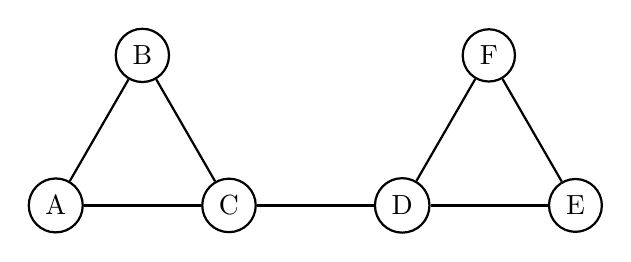
\begin{tikzpicture}[node distance=2cm, scale=1.1]
                \begin{scope}[every node/.style={circle,thick,draw}]
                    \node (A) at (0, 0) {A};
                    \node (B) at (1, 1.7320508076) {B};
                    \node (C) at (2, 0) {C};
                    \node (D) at (4, 0) {D};
                    \node (E) at (6, 0) {E};
                    \node (F) at (5, 1.7320508076) {F};
                \end{scope}

                \draw[black, thick] (A) -- (B);
                \draw[black, thick] (A) -- (C);
                \draw[black, thick] (C) -- (B);
                
                \draw[black, thick] (C) -- (D);

                \draw[black, thick] (D) -- (E);
                \draw[black, thick] (D) -- (F);
                \draw[black, thick] (E) -- (F);
            \end{tikzpicture}
            \caption{Graph abstraction of possible circuit}
            \label{fig:example-circuit-traversal}
        \end{figure}

        The general idea with this new approach is that whenever there is a split (i.e. a node), then the program has two paths to choose from to continue on. 
        In \autoref{fig:example-circuit-traversal}, there is a fork at C that leads to either B or D. 
        The program will first try going from C to B, and then attempt to reach C again while not traversing an edge twice/visiting the same vertex twice, for example it can go through A and then back to C, and it would know that B is connected to the main circuit, and so it would receive a current.
        However, when it tries to make it back to C after traversing CD following the same rules, then it fails to make it back to C. 
        After some thought, the best method discovered was a brute-force search by exhaustion. From D the program would then choose between E and F, suppose it choose E first. 
        Then from E it would have to go to F, and then from F there would be no open paths to take, and so it would back-traverse to the last choice and make a different one, in this example it would choose to go from D to F, and then it would go to E, and then again it would realise there are no available paths to choose from. 
        This would then complete the search by exhaustion showing that the vertices beyond C in the direction of D are in fact not connected to the main circuit, and thus could be ignored.
        In order to keep track of which vertices have been visited, a dynamic data structure could be used such as the Python list. 
        
        The main disadvantage with this approach is that it is anticipated to be slow, however with smaller circuits there is hope that the program will be able to run at a satisfactory rate. 

        There is also the issue with available development time. 
        Considering how much more complex the program will be when including the node component, it may be a viable option to release the software without this capability and then add it in an update later on in the lifetime of the software. 

        % So glad the final final non-negotioable deadline is, infact, negotiable. 
        % But if i'm honest, I dont want to work on this beyond january whatsoever, so I will try to complete it

        
    \subsection{User Interface}

        The user interface in this cycle will consist of the user being able to interact with circuits. 
        This refers to them being able to create circuits as well as them being able to read data from the circuits.

        % fig:ui-create-circuits-design
        % User interface allowing user to create circuits design
        \begin{figure}[!ht]
            \centering
            \includegraphics[width=.7\textwidth]{s05/design/user-interface-make-circuits.png}
            \caption{User interface allowing user to create circuits design}
            \label{fig:ui-create-circuits-design}
        \end{figure}

        Shown in \autoref{fig:ui-create-circuits-design} is the design for a user being able to interact with creating circuits. 
        On the top is a ribbon that contains commands related to the program. 
        From the `File' tab, the user will be able to save, close, open projects, and the `Options' tab will include options to simulate the circuit and other miscellaneous commands. 
        
        On the right side is an area that the user will be able to select circuit components onto and ultimately build their circuit, referred to as the `canvas'. 
        Notice how the canvas contains lattice points, these will be used as anchor points for the components, and a connection can only be made when two terminals overlap on a point. 
        The user will be able to click on a component, contained on the left-hand side, and then click on two different lattice points that determine where the terminals for the component lie. 
        For consistency, the first lattice point to be clicked on will be the positive terminal, and the second one the negative terminal. 
        Then the canvas will contain a render of the selected component connected to the appropriate lattice points.

        The other way that the user will interact with the circuits is through reading off data from them.
        When the user places a voltmeter or ammeter, they will first be shown a menu that allows them to configure the meter, shown in \autoref{fig:ui-ammeter-config-design}. 
        This allows the user to choose a suitable identifier (chosen to be limited to 12 characters, to make sure that it fits properly in later use), the units (e.g. amperes, milliamperes, etc.), which are chosen from a dropdown menu, and the amount of significant figures that the readings are shown to, limited to eight, with buttons that allow them to increment or decrement this value. 
        After setting these values up, the user can place the ammeter like a normal component. 

        % fig:ui-ammeter-config-design
        % User interface to configure an ammeter
        \begin{figure}[!ht]
            \centering
            \includegraphics[width=.7\textwidth]{s05/design/user-interface-init-meter.png}
            \caption{User interface to configure an ammeter}
            \label{fig:ui-ammeter-config-design}
        \end{figure}

        After the user chooses to run the circuit, they are shown the interface in \autoref{fig:ui-meter-readings-design}. 
        A key difference in this interface is that the font is monospaced, meaning that every character has the same width.
        This makes it easier for the user to read the numbers as they are also all aligned with each other. 
        There is a space between the units and the values, and the units are given two characters of space. 
        This also improves readability as all the characters aren't packed as densely together. 
        `Ammeter1', `Ammeter2', and `Voltmeter1' will be replaced with the user-given identifiers that they decide with the menu in \autoref{fig:ui-ammeter-config-design}. 

        % fig:ui-meter-readings-design
        % User interface to allow the user to read off the meters
        \begin{figure}[!ht]
            \centering
            \includegraphics[width=.7\textwidth]{s05/design/ui-meter-readings-design.png}
            \caption{User interface to allow the user to read off the meters}
            \label{fig:ui-meter-readings-design}
        \end{figure}

        % Talk about which success criteria im skipping out on 
        % I think i do that later though 


\newpage
\section{Testing}

    The testing table is shown in \autoref{tbl:test-data-cycle3}.

\section{Implementation}


    % Making frames

    As in previous cycles, the GUI element is implemented as a class with the various widgets being methods and attributes to that class. The code for initialising the size of the window is shown in \autoref{sc:simgui-init}. 

    The idea of `Frames' from the Tkinter library to divide content, as specified in the design of this cycle, has been used in the user-interface. 
    The code for the frames is shown in \autoref{sc:simgui-frames-example}, and the output is shown in \autoref{fig:frames-proof}. 
    Note that the colours are temporary and are only used here to make it clear where the frames are. 

    % fig:frames-proof
    % Frames to divide content
    \begin{figure}[!ht]
        \centering
        \includegraphics[width=.7\textwidth]{s05/implement/simgui-frames.png}
        \caption{Frames to divide content}
        \label{fig:frames-proof}
    \end{figure}


    % Lattice points placing and stuff

    In order to allow the user to click on the lattice points, the iterative placing of buttons onto the grid was needed. 
    The idea is that buttons will be placed using an iterative for loop, and when a button was pressed it would return its position on the grid which would allow for it to be identified. 
    The code for placing the buttons and initialising the commands for the buttons is shown in \autoref{sc:simgui-placing-canvas-buttons}.
    For this implementation, the Python lambda functionality had to be used, with which I had not had previous experience. 
    In order to learn how to use it in this scenario, I had used the website W3Schools to learn more about the syntax and functionality of how to use it, and an answer on StackOverflow which the link to which is in a comment in the code listing. 
    The \verb|index| variable is important in this implementation as it signifies the order of when a given button was placed, incrementing by one after each button. 
    By knowing how many buttons there are in each row and column, it is possible to calculate the position of the button from just the index. 
    A method to return and print the index is shown in \autoref{sc:simgui-return-index-method}.
    Evidence for this working is shown in \autoref{fig:buttons-index-output-pf}. 

    % fig:buttons-index-output-pf
    % Evidence for buttons printing their index
    \begin{figure}[!ht]
        \centering
        \includegraphics[width=.7\textwidth]{s05/implement/buttons-index-working.png}
        \caption{Evidence for buttons printing their index}
        \label{fig:buttons-index-output-pf}
    \end{figure}

    In order to make the buttons small and square, an image had to be used due to the way sizing works in the GUI module used. 
    In Tkinter, if you specify the height of a button, it is specified as multiples of the height of the character \verb|0|. 
    Likewise, if you specify the width of a button it also uses multiples of the width of the character \verb|0|. 
    This makes it difficult/impossible to make buttons square with any given side length.
    The solution is to create an image that has the desired dimensions and then specify that as the image used for the button. 
    For this the file \verb|lattice.png| was used, which is a 5 pixel tall and 5 pixel wide image containing only black pixels. 
    However, I don't believe that the program would actually use the image for the button, it just allowed me to specify the height and width in pixels, as I still had to specify the background colour of the button as `black' in the declaration of each button. 
    Furthermore, trying to access the heights and widths of the \verb|PhotoImage| object both returned 0 where I would expect it to return 5 for both. 
    
    One initial problem was with the spacing and layout of these lattice points. 
    As shown in \autoref{fig:grid-spacing-wrong}, the spacing was inconsistent due to not taking into account the size of the buttons themselves. 

    % fig:grid-spacing-wrong
    % Incorrect button spacing around borders
    \begin{figure}[!ht]
        \centering
        \includegraphics[width=.7\textwidth]{s05/implement/grid-spacing-wrong.png}
        \caption{Incorrect button spacing around borders}
        \label{fig:grid-spacing-wrong}
    \end{figure}

    One solution that slightly improved this on this issue was shifting the positions of the buttons to the left and upwards by the width and height of the buttons respectively. 
    The result of this is shown in \autoref{fig:improved-button-spacing-pf} and the improved code is shown in \autoref{sc:simgui-improved-button-placing}. 

    % fig:improved-button-spacing-pf
    % Improved button spacing
    \begin{figure}[!ht]
        \centering
        \includegraphics[width=.7\textwidth]{s05/implement/grid-spacing-improve1.png}
        \caption{Improved button spacing}
        \label{fig:improved-button-spacing-pf}
    \end{figure}


    % Component buttons

    Next the buttons allowing components to be selected were implemented.
    Initially, the text on the buttons would not show.

    % fig:no-text-on-components
    % Text not showing on buttons
    \begin{figure}[!ht]
        \centering
        \includegraphics[width=.7\textwidth]{s05/implement/no-button-text-showing-pf.png}
        \caption{Text not showing on buttons}
        \label{fig:no-text-on-components}
    \end{figure}

    I had thought that the problem lied with the variables inside the loop, as there was a similar problem with getting the commands attached to the buttons to work, however when declaring it with a constant string the text still would not show.
    This attempt is shown in \autoref{fig:no-text-on-components-const-string}.

    % fig:no-text-on-components-const-string
    % Text still not showing when using constant string
    \begin{figure}[!ht]
        \centering
        \includegraphics[width=.7\textwidth]{s05/implement/no-button-text-02.png}
        \caption{Text still not showing when using constant string}
        \label{fig:no-text-on-components-const-string}
    \end{figure}

    The issue seemed to come from using the trick of setting the image attribute in order to be able to set the dimensions of the button in pixels.
    After removing the image attribute and setting the size when calling the \verb|place| method, the text showed on the buttons as wanted. 
    The code for the lattice points from before was also changed to no longer use the image attribute in order to stay consistent. 
    The code is shown in \autoref{sc:simgui-component-buttons} and evidence for the code working is shown in \autoref{fig:component-buttons-text-working}. 

    % fig:component-buttons-text-working
    % Text showing corrently on component buttons
    \begin{figure}[!ht]
        \centering
        \includegraphics[width=.7\textwidth]{s05/implement/component-buttons-text-working.png}
        \caption{Text showing currently on component buttons}
        \label{fig:component-buttons-text-working}
    \end{figure}


    % Ribbon buttons

    The final buttons to be placed were there to allow the user to interact with the project. 
    These allow the user to save and exit the project. 
    They are shown in \autoref{fig:save-and-quit-buttons-placed}.

    % fig:save-and-quit-buttons-placed
    % Save and quit buttons placed
    \begin{figure}[!ht]
        \centering
        \includegraphics[width=.7\textwidth]{s05/implement/save-and-quit-buttons-placed.png}
        \caption{Save and quit buttons placed}
        \label{fig:save-and-quit-buttons-placed}
    \end{figure}


    % Removing frame colours

    Now that all the buttons have been placed, the frames can be properly formatted without the background colours. 
    After removing the background colours and adding in relief styles in order to make the sections discernable from each other the user interface looks like in \autoref{fig:simgui-final-look}.

    % fig:simgui-final-look
    % Final GUI layout
    \begin{figure}[!ht]
        \centering
        \includegraphics[width=.7\textwidth]{s05/implement/final-simgui-look.png}
        \caption{Final GUI layout}
        \label{fig:simgui-final-look}
    \end{figure}


    % Ammeter creation ui

    Next the user interface to allow the user to configure the meter was created.
    The final result is shown in \autoref{fig:metergui-final}. 
    Again, the use of variables in order to place components was used which results in a more consistent look which improves readability and usability. 
    The initialisation of the user interface is done in \autoref{sc:metergui-init}.

    The code to place the entry and label for the identifier is shown in \autoref{sc:metergui-id-lbl-ent}.
    This time for validation, the \verb|validate| and \verb|validatecommand| arguments were passed as attributes to the initialisation of the entry. 
    This will make it so that text that doesn't pass validation cannot even be entered in the first place, which is a more robust solution than before, which relied on getting the values after the user had already entered them. 
    The function that validates an identification string is shown in \autoref{sc:id-validation-func}. 

    The code to create the dropdown selection for the units is shown in \autoref{sc:metergui-units-lbl-menu}. 
    Validation isn't necessary for this, as the dropdown limits the user to only valid inputs. 

    The code to place the entry and label for the resolution is shown in \autoref{sc:metergui-res-lbl-ent}.
    Again validation is implemented through Tkinter, and the function for validation is shown in \autoref{sc:resolution-validation-func}. 

    The code for placing the `Create' button is shown in \autoref{sc:metergui-create-btn}. 
    This button will finalise the creation of the ammeter and will pass the data onto the main program. 

    % fig:metergui-final
    % MeterGUI user interface
    \begin{figure}[!ht]
        \centering
        \includegraphics[width=.7\textwidth]{s05/implement/metergui-final.png}
        \caption{MeterGUI user interface}
        \label{fig:metergui-final}
    \end{figure}

    The command for the `Create' button is shown in \autoref{sc:metergui-create-btn-command}. 
    This makes use of global variables, as both the \verb|MeterGUI| and \verb|SimulatorGUI| are written in the same file, so they share the variable \verb|meter|. 
    Since empty results are not valid but pass the previous validation checks, a final check for empty inputs is done here. 
    The data is put into the global dictionary and the window terminates. 

    
    % Talking about the flags with the lattice buttons and component buttons

    After the user selects a component by pressing one of the buttons on the left, they are then allowed to select two unique lattice points that represent the positive and negative terminals of their component. 
    There was difficulty figuring out logic for how information would be shared between the buttons, particularly because the buttons were defined iteratively meaning that there wasn't an easy way to reference them. 

    Firstly, flags were declared inside the \verb|__init__| method of the \verb|SimulatorGUI| class, shown in \autoref{sc:simgui-declare-flags}. 
    The \verb|active| flag is set to `True' when the user selects a component, which then allows them to select two lattice points. 
    The \verb|pos| and \verb|neg| attributes are declared as Tkinter \verb|IntVar|s, which is important as it allows for functionality in the command for the component button. 
    These are initialised to -1, which is a value they would not be able to attain from user input. 
    
    The command for the lattice point buttons was updated, shown in \autoref{sc:simgui-lattice-btn-command-real}. 
    It checks for the \verb|active| flag, and does nothing if it is set to \verb|False|. 
    Then it sets the values for \verb|pos| and \verb|neg| in that order, by checking which is left to be set to a value other than -1. 
    An extra check is made to prevent the user from pressing the same button twice. 


    % Component buttons
    
    The code for the component buttons is shown in \autoref{sc:simgui-comp-btn-cmd}. 
    The first thing to check is whether another component is already being placed, in which case the method stops processing further.
    This is in order to allow for only a single component to be placed at any one time. 
    Then the \verb|active| flag is set to \verb|True| to show that a component is being placed. 
    Since meters are treated as a special case with the extra user interface window, there is a check to see whether the current component is a meter. 
    The code for the button cannot proceed if \verb|neg| has not been set to a value by the user, i.e. if the user has not selected two points for the terminals. 
    The information taken from the user is placed into the \verb|component| dictionary, the flags are reset and the component is added to another dictionary called \verb|circuit| which stores all the components placed by the user. 


    % Ribbon buttons code

    Next, functionality for the buttons on the top ribbon was tackled. 


    % Quit button 

    The quit button is an alternative to the `X' in the top right corner of the window. 
    It closes the window and does no further processing. 
    The code for it is shown in \autoref{sc:simgui-quit-btn-command}. 


    % Reset button

    The reset button was similarly simple. 
    It sets the \verb|circuit| dictionary to an empty dictionary to reset the circuit.
    The code for it is shown in \autoref{sc:simgui-reset-btn-command}.

    
    % Save button

    The purpose of the save button is to write the \verb|circuit| attribute to a JSON file in the format shown in \autoref{ps:json-proj-config-example}. 
    The method starts with \autoref{sc:simgui-save-cmd-1}, by declaring an empty dictionary that will be the one written to the JSON file using the JSON library, as well as looping over every component in the \verb|circuit| attribute in order to find out which components are connected to which by checking which share a terminal. 

    %   Looking for connected terminals

    This was done by looping over the components again, making sure to avoid checking against itself.
    The variable \verb|single| is kept and incremented whenever a component that shares terminals is found. 
    Since only two components can share a lattice point, then this raises an error if more than one is found, and if none are found that implies an incomplete circuit, so an error is also raised. 
    The circuit also resets itself if these occur, as that is currently the only way for the user to undo anything. 
    A similar process is repeated for searching for connections to the negative terminals.
    The code for each is shown in \autoref{sc:simgui-save-cmd-2} and \autoref{sc:simgui-save-cmd-3} respectively. 

    %   Saving rest and writing to JSON

    Finally, the `type' and `data' values were copied directly from the \verb|circuit| attribute without the need for further processing, and the \verb|jsonCircuit| dictionary is written to a file called \verb|circuit.json| with the use of a custom procedure shown in \autoref{sc:dict2json-procedure}. 
    This final step is shown in \autoref{sc:simgui-save-cmd-4}. 

    An example output is shown in \autoref{fig:save-button-example-output}.

    % fig:save-button-example-output
    % Example output of `Save' button
    \begin{figure}[!ht]
        \centering
        \includegraphics[width=.7\textwidth]{s05/implement/circuit-json-example.png}
        \caption{Example output of `Save' button}
        \label{fig:save-button-example-output}
    \end{figure}


    % Run button

    Finally, the `Run' button was implemented, which is responsible for getting readings from the ammeters to the user. 

    %   OutputGUI
    
    There is a user interface window that is shown during the `Run' button's process, the initialisation of which is shown in \autoref{sc:outputgui-init}. 
    Note that this also takes the dictionary \verb|readings| as a parameter.
    This stores information about the circuit, such as total resistance and E.M.F. as well as the readings from each meter in the circuit, an example is shown in \autoref{pc:readings-dict-example}. 
    For alignment purposes, all the strings are made to the same length using the custom function \verb|normaliseString| shown in \autoref{sc:normalise-string-function}. 
    It was decided to make this into a function since it was repeated many times in this section. 

    % pc:readings-dict-example
    % Example readings dictionary
    \begin{figure}[!ht]
        \inputminted[linenos]{json}{figures/s05/implement/data.json}
        \caption{Example readings dictionary}
        \label{pc:readings-dict-example}
    \end{figure}

    Then the program loops over each ammeter found and adjusts their readings to take account for units as well as significant figures, using a custom function to round a number to a given number of significant figures shown in \autoref{sc:sigfigs-function}. 
    The code is shown in \autoref{sc:outputgui-loop}, and an example output is shown in \autoref{fig:outputgui-example-output}.

    % fig:outputgui-example-output
    % Example output from OutputGUI
    \begin{figure}[!ht]
        \centering
        \includegraphics[width=.7\textwidth]{s05/implement/output-gui-awesome.png}
        \caption{Example output from OutputGUI}
        \label{fig:outputgui-example-output}
    \end{figure}

    %   Ammeter check

    The actual method starts in \autoref{sc:simgui-meter-check} by first reading the result from the previous `Save' button into a Python dict using a custom function shown in \autoref{sc:json-to-dict-function}. 
    It also does quick-return check for whether there are any meters in the circuit, as if there are no meters then there is also no output, which means no computation has to be done. 
    This saves on computation time as well as dealing with edge cases where there are no meters in the circuit. 

    %   Total current calculation

    Since there are only ammeters in these circuits and since all the circuits are made in series then the calculation for the ammeter reading is relatively easy.
    Using Ohm's Law, \[ V = IR, \] we can rearrange for current to give \[ I = \frac{V }{R } = \frac{\Sigma V }{\Sigma R}, \] so all we need for the current is to sum all the electro-motive forces and resistances for all the components and divide one by the other. 

    Since user input for component values hasn't been implemented, the data for the components is stored in a JSON file that is read from whenever the circuit is run, which is shown in its entirety in \autoref{sc:data-json-components}. 
    Importantly, the keys of this JSON file match to the value of the `type' key in the \verb|data| sub-dictionary that is used to store components in the circuit.
    This makes it easy to fetch the information about a component, which is what is done in the for loop of \autoref{sc:simgui-run-command-total-current}. 
    There is a final check for if the user hasn't placed components with non-zero resistance, as that would lead to a division by zero. 

    %   Ammeter list

    Finally, the list of ammeters is created by once-more looping over all the components in the circuit, this time making sure to ignore any non-meter components.
    An extra entry is made to store the reading of the meter before they are passed to the aforementioned \verb|OutputGUI|.

\section{Evaluation}
    The implementation so far is now going to be evaluated against the success criteria declared at the beginning of this cycle, shown in \autoref{tbl:succ-crit-c3}. 

    \textbf{Analysis of success criteria:}
    \begin{itemize}
        \item A1: Model electric circuits accurately
        \begin{itemize}
            \item Partially achieved
            \item Mostly accurate, apart from the program currently ignoring polarity of cells. Normally two opposing cells with E.M.F. of 12 V would result in 0 V E.M.F., but in this implementation it results in 24 V of E.M.F. Parallel circuits are also not available as of this implementation.
        \end{itemize}
        \item A2: Be able to handle 10 or fewer components in a single circuit
        \begin{itemize}
            \item Achieved
            \item The circuit can handle many components
        \end{itemize}
        \item A3: Have support for at least the following components: cell, wire, filament bulb, resistor, multimeter, switch. Each should have respective attributes be customisable.
        \begin{itemize}
            \item Partially achieved
            \item All but the switch and voltmeter components have been implemented, and the only customisable component is the ammeter. User input has been moved to a later development cycle.
        \end{itemize}
        \item A4: Have general attributes of the circuit displayed, such as total resistance, current, potential difference, and electro-motive forces
        \begin{itemize}
            \item Partially achieved
            \item All but potential differences of components has been implemented, due to parallel circuits, and therefore voltmeters, not being implemented
        \end{itemize}
        \item A6: An intuitive way to add components to a circuit, most likely being able to drag components onto the main stage using the mouse
        \begin{itemize}
            \item Achieved
            \item The user is able to select a component and then select two terminals to show where it connects
        \end{itemize}
        \item A7: Charge flow indicator to visualise charge flow around the circuit. Toggle between electron flow, conventional current, and off. 
        \begin{itemize}
            \item Not achieved
            \item This was not achieved, and neither was the visualisation of the circuits the user creates. 
        \end{itemize}
        \item A8: Nameable components for easier management
        \begin{itemize}
            \item Partially achieved
            \item Ammeters are nameable, but the rest of the components are not. 
        \end{itemize}
    \end{itemize}

    A lot of functionality has been moved to a future cycle, particularly regarding user inputs and outputs, as well as the ability to create circuits in parallel. 


    % To Do:
    %   - Hierarchy diagram
    %   - Do more testing
